\documentclass{article}
\usepackage[minionint,mathlf,textlf]{MinionPro} % To gussy up a bit
\usepackage[margin=1in]{geometry}
\usepackage{graphicx} % For .eps inclusion
%\usepackage{indentfirst} % Controls indentation
\usepackage[compact]{titlesec} % For regulating spacing before section titles
\usepackage{adjustbox} % For vertically-aligned side-by-side minipages
\usepackage{array, mathrsfs, mhchem, amsmath} % For centering of tabulars with text-wrapping columns
\usepackage{hyper ref}
\usepackage[autolinebreaks,framed,numbered]{mcode}
\pagenumbering{gobble} 
\setlength\parindent{0 cm}
\begin{document}
\large

\section*{Motivation for stochastic modeling}

\begin{itemize}
\item At the beginning of this course, we warned that there would be an emphasis on determinism. This choice was motivated by a desire to keep the math prerequisites minimal and, particularly, within the department's undergraduate requirements. (Differential equations, but not probability and statistics, is required for Molecular and Cellular Biology concentrators.) We now discuss whether these deterministic methods are appropriate.
\item For a sense of scale, consider the \textit{E. coli} cell: roughly one micron in length and one femtoliter in volume. The dry mass of protein in this cell is approximately 0.15 picograms ($1.5 \times 10^{-13}$ grams).
\item An average protein is about 300 amino acids in length. A typical amino acid weighs about one hundred Daltons (g/mol). Therefore, a single protein weighs about 30,000 g/mol = $5 \times 10^{-20}$ grams. This means that we expect about $3 \times 10^{6}$ proteins per cell.
\item \textit{E. coli} has roughly five thousand genes, so on average 600 proteins per gene. The Xie lab (Taniguchi et al., 2010) has quantified average protein and transcript number, revealing that many have an average number of ten or fewer copies per cell.
\end{itemize}
\begin{center}
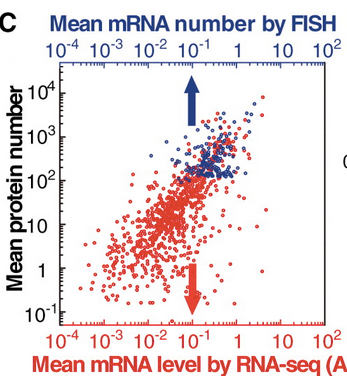
\includegraphics[width=0.3\textwidth]{xie_2010.png}
\end{center}
\begin{itemize}
\item The average mRNA number per cell is less than one for the majority of the genes examined. In a large population some cells have no mRNAs, while others have one or more. In principle this could reflect determinism: for example, subsets of cells might enter different states of a bistable switch due to differences in the environment experienced by their ancestors. 
\item However given the genetic and environmental similarity of the populations used for this experiment, the more natural expectation is an ergodic one, i.e. that the population average at one time represents the time-averaged behavior of a single cell, and therefore that individual cells are losing and gaining mRNAs over time. Deterministic trajectories like limit cycles or chaotic behavior could still explain variation over time, but not parsimoniously.
\item An alternative explanation invokes the notion of a stochastic system, i.e. one in which there are multiple (probably infinite) possible trajectories along which a system can evolve from any initial condition. Is this explanation defeatist or appropriate?
\item Justification lies with the nature of chemical reactions. It is good sense that a reaction cannot proceed without consuming and producing whole numbers of its reactants and products. Furthermore, reactions occur at discrete moments in time: they are not happening continuously as the mass action rate laws we have dutifully consulted would seem to imply.
\item If we return to our assumptions, we will find that the law of mass action was never intended to be applied when the number of molecules in a system is low or when the system is not well-mixed. However, low copy numbers and spatial inhomogeneity are frequently a reality in biological systems.
\item The types of deterministic models we have been using to date do not account for those effects, but you might argue that if we knew the structures and initial positions and momenta for every molecule, that we ought to be able to combine these with what we know of the physical forces of Nature to model how the system will evolve. But even this intuition is wrong, since we cannot know both position and momentum with arbitrary accuracy; quantum mechanics denies us certainty in many other aspects, too.
\item This does not mean we should despair, because there is a lot that we can understand about a system statistically even if we cannot predict its behavior absolutely.
\end{itemize}

\section*{A few words about noise}
\begin{itemize}
\item Before jumping in, it's worthwhile to consider where the noise -- i.e. those indeterminate effects that force us to resort to stochastic models -- is coming from. The Heisenberg uncertainty principle is not a realistic starting point for the description of our woes.
\item Molecules in solution are randomly buffeted by collisions with solvent molecules, whose positions and momenta we have no hope of knowing, so that even a molecule's flight path is not predictable. From this we see that the time until two molecules collide with one another -- a necessary prerequisite for many reactions -- is variable. We'll discuss this subject in more depth in a later lecture on diffusion, which will serve as our sole foray into the world of stochastic differential equations. (Briefly mention where diffusion fits into the Arrhenius rate law here.)
\item Diffusion is slow and may not be directed: in cases where this is not acceptable (e.g. transport down a long axon) energy-dependent directed transport is possible instead.
\item Another major source of noise, when copy number is low, is the distribution of molecules upon division. A cell with ten copies of a protein has a non-negligible chance of forming a septum in such a way that one daughter cell receives no copies at all.
\item In some cases, this noise in partitioning must be avoided. Low copy number essential components, such as the genome and MTOCs, are actively segregated at cell division.
\item Many other examples are possible, but a shared point is that when noise in a system cannot be tolerated, solutions do exist for exercising more control over outcomes. (You'll study a simple one -- your old friend, negative autoregulation -- on your upcoming problem set.) If those mechanisms have not evolved in a natural biological system, we might assume their energetic costs outweigh their benefits $\ldots$ with the usual caveats.
\item On the other hand, proper functioning of some biological systems \textit{relies} on non-deterministic behaviors. On your next homework, you'll study a model system whose deterministic solution is stable but which exhibits oscillations when we account for the discrete nature of reactions and entities in the system. You'll also see a few examples within the next two sections of the course, which we won't spoil now.
\end{itemize}

\section*{Stochastic modeling notation}
\begin{itemize}
\item The first problem we encounter when attempting to keep track of the absolute number of molecules of each species is that the reaction rates scale with \textit{concentrations}, not molecule number. To switch back and forth between concentrations and molecule numbers, we will need to introduce a system volume, which is traditionally denoted by $\Omega$.
\item We will assume that a chemical reaction system has $N$ different molecular species. The number of molecules of each species at any given time is the state vector $\mathbf{X}(t) = (X_1, \ldots, X_N)^T$. The number of molecules at a given time is no longer given deterministically: we therefore consider the $X_i$s to be random variables.
\item The system experiences $M$ reactions. $\mathbf{s}_j$ is the stoichiometry vector for reaction $j$: you first encountered these in week two, when we discussed moiety conservation. Together these stoichiometry column vectors make up the stoichiometry matrix, $\mathbf{S} = [\mathbf{s_1}, \ldots,  \mathbf{s_M}]$.
\item When the $i$th reaction occurs, the state vector changes slightly from $\mathbf{X}$ to $\mathbf{X} + \mathbf{s}_i$.
\item We denote the rate of reaction $j$ by $ \Omega\, r_j(\mathbf{X},\Omega)$. The notation helps us to remember that mass action reaction rates actually depend upon the concentrations $\mathbf{X}(t)/\Omega$, and return rates of change in concentration per unit time, which we need to convert back to molecule number per unit time by multiplying the output by $\Omega$\footnote{Some authors do not write this notation out explicitly. You will also find some cases where the argument to $r$ is simply $\mathbf{X}/\Omega$ -- however, this does not work so well when molecule number is small and we have bimolecular reactions, as you will see in an example later in this lecture.}. For example:
\[ \ce{X ->[k] \varnothing} \hspace{2 cm} \Omega r(X, \Omega) = \Omega \left[ k \left( \frac{X}{\Omega} \right) \right] = kX \textrm{ as usual} \]
\end{itemize}

\section*{Chemical master equation}
\begin{itemize}
\item Let $P(\mathbf{X},t)$ be the probability that the system will have the state vector $\mathbf{X}$ at time $t$.  To learn how this probability distribution will change in time, we consider what changes are possible during a time interval $dt$ so short that we can be reasonably confident that either exactly one reaction occurs or no reactions occur at all.
\item Under this assumption, there are two ways that the system can find itself in state $\mathbf{X}$ at time $t+dt$:
\begin{itemize}
\item The system was in state $\mathbf{X}$ at time $t$, and no reactions occurred. Multiplying the probabilities of these two independent events together, we get that the likelihood of this is $P(\mathbf{X},t) \left[ 1 - \Omega \sum_{j=1}^M r_j(\mathbf{X}, \Omega) \, dt \right]$.
\item The system was in one of the $M$ ``neighboring" states $\mathbf{X} - \mathbf{s}_j$ at time $t$, and then reaction $j$ occurred. The probability of these two occurrences, summed over all $M$ reactions, is $\Omega \sum_{j=1}^M P(\mathbf{X} - \mathbf{s}_j) r_j (\mathbf{X} - \mathbf{s}_j,\Omega) \, dt$.
\item The probability that two reactions occur during this short time, which scales with $(dt)^2$, is taken to be negligible.
\end{itemize}
\item Then we can express the updated probability distribution by:
\[ P(\mathbf{X},t+dt) \approx P(\mathbf{X},t)  - \Omega P(\mathbf{X},t)  \sum_{j=1}^M r_j(\mathbf{X},\Omega) \, dt  + \Omega \sum_{j=1}^M P(\mathbf{X} - \mathbf{s}_j) r_j (\mathbf{X} - \mathbf{s}_j, \Omega) \, dt \]
\item Subtracting $P(\mathbf{X},t)$ from both sides, dividing by $dt$ and taking the limit as $dt \to 0$, we arrive at an expression called the \textit{chemical master equation}:
\[ \frac{dP(\mathbf{X},t)}{dt} =   \Omega \sum_{j=1}^M \left[ P(\mathbf{X} - \mathbf{s}_i) r_j (\mathbf{X} - \mathbf{s}_j, \Omega)  - P(\mathbf{X},t) r_j(\mathbf{X}, \Omega)  \right] \]
\item To simplify this expression, we introduce the step operator $\mathbb{E}$. The step operator adds the value denoted in superscript to the $i$th argument of any function it acts upon. For example,
\begin{eqnarray*}
P(\mathbf{X}-\mathbf{s}_j,t) r_j(\mathbf{X}-\mathbf{s}_j,\Omega) = P\left( \begin{bmatrix} X_1 - S_{1j}\\ \vdots \\ X_N - S_{Nj} \end{bmatrix}, t \right) r_j\left( \begin{bmatrix} X_1 - S_{1j}\\ \vdots \\ X_N - S_{Nj} \end{bmatrix}, \Omega \right) = \left[ \prod_{i=1}^N \mathbb{E}^{-S_{ij}} \right] P(\mathbf{X},t) r_j(\mathbf{X},\Omega) 
\end{eqnarray*}
\item This allows us to rewrite the chemical master equation as:
\[ \frac{dP(\mathbf{X},t)}{dt} =   \Omega \sum_{j=1}^M \left[ \prod_{i=1}^N \mathbb{E}^{-S_{ij}} - 1 \right]  P(\mathbf{X},t) \, r_j (\mathbf{X}, \Omega)  \]
\item If the number of states is finite, then we could attempt to find fixed points by setting all time derivatives equal to zero as we usually have. You will try this out on problem set 7. However, in general the number of possible states is infinite, and we need other methods to learn about the probability distribution of system states.
\end{itemize}

\section*{Example: Irreversible dimerization (Paulsson, 2013)}
\begin{itemize}
\item By way of illustration, let's consider a simple system with one molecule, $X$, and two reactions. We'll imagine $X$ to be a protein that is produced at a constant rate but irreversibly forms dimers:
\[ \ce{\varnothing {\color{white}.} ->[k_1] X} \hspace{2 cm} \ce{2X ->[k_2] \varnothing} \]
\item Our stoichiometry matrix and reaction rate functions are:
\[ \mathbf{S} = \begin{pmatrix} 1 & -2 \end{pmatrix} \hspace{1 cm} r_1(x,\Omega) = k_1  \hspace{1 cm} r_2(x,\Omega) = k_2 \left( \frac{x}{\Omega} \right) \left( \frac{x - 1}{\Omega} \right) \]
Notice how the reaction rates use $\Omega$ to convert the number of molecules into a concentration. Also notice that in the bimolecular interaction we have been careful to account for the discreteness of $x$.
\item We have everything we need now to plug into our formula for the chemical master equation:
\begin{eqnarray*}
\frac{dP(x,t)}{dt} & = & \Omega \sum_{j=1}^M \left[ \mathbb{E}^{-S_{1j}} - 1 \right]  P(x,t) \, r_j (x, \Omega)\\
& = & \Omega \left[ P(x-S_{11},t) \, r_1(x-S_{11},\Omega) - P(x,t) \, r_1(x,\Omega) + P(x-S_{12},t) \, r_1(x-S_{12},\Omega) \right.\\
& & \hspace{1 cm} \left. - P(x,t) \, r_2(x,\Omega) \right]\\
& = & k_1 \Omega P(x-1,t) + \frac{k_2}{\Omega}(x+2)(x+1) P(x+2,t) - \left[ k_1 \Omega + \frac{k_2}{\Omega} x(x-1) \right] P(x,t)
\end{eqnarray*}
\item We promised that the course would not assume a background in statistics, but know that the mean and variance of a discrete, non-negative variable is calculated as follows:
\[ \left< x^n \right> = \sum_{x=0}^{\infty} x^n P(x) \hspace{2 cm} \mu = \left< x \right> \hspace{ 2 cm} \sigma^2 = \left< x^2 \right> - \left< x \right>^2 \]
\item The chemical master equation allows us to calculate a related quantity: the change in the average number of molecules with time. We can split into separate sums and shift $x$ as necessary to proceed with the calculation:
\begin{eqnarray*}
\frac{d \left< x \right>}{dt} = \sum_{x=0}^{\infty} x \frac{dP(x,t)}{dt} & = & k_1 \Omega \sum_{x=0}^{\infty} x P(x-1,t) + \frac{k_2}{\Omega} \sum_{x=0}^{\infty} x(x+2)(x+1)P(x+2,t)  \ldots\\
& = & k_1 \Omega \sum_{x=0}^{\infty} (x+1)P(x,t) + \frac{k_2}{\Omega} \sum_{x=0}^{\infty} x(x-2)(x-1)P(x,t)  + \ldots\\
& = & k_1 \Omega \left< x + 1\right> + \frac{k_2}{\Omega} \left< x(x-1)(x-2) \right> - k_1 \Omega \left< x \right> - \frac{k_2}{\Omega} \left< x^2(x-1) \right> \\
& = & k_1 \Omega  -\frac{2 k_2}{\Omega} \left< x(x-1) \right>
\end{eqnarray*}
Notice that we can take advantage of the linearity of the average and derivative operators to commute them around one another in the first and final lines.
\item The variance in $x$ is $\sigma_x^2 \triangleq \left< x^2 \right> - \left< x \right>^2$, so we can rewrite the result above as
\[ \frac{d \left< x \right>}{dt} = k_1 \Omega - \frac{2 k_2}{\Omega} \left( \sigma_x^2  + \left< x \right>^2 - \left< x \right> \right) \]
\item This rate can be set equal to zero and solved to find the steady-state value of $\left< x \right>$. You'll notice, though, that this will depend on the variance and the volume of the system -- two things which have never appeared in our results before. You will probably be surprised to learn that the average can depend on the variance, but in fact this is the general case when rates are nonlinear (e.g. for bimolecular reactions, Michaelis-Menten kinetics, etc.). It is not uncommon either to find that each moment is defined in terms of larger moments, so that we cannot find a closed expression for the moments. (A technique which we will not cover but which is briefly mentioned in the readings, called moment closure, can address this issue.)
\item When mean and variance can be calculated or measured, a few metrics exist for comparing the \textit{dispersion} of the distribution. The most commonly used are the Fano factor, $\sigma^2/\mu$, and the coefficient of variation, $\sigma/\mu$. The Poisson distribution has Fano factor 1 regardless of the parameter:
\begin{eqnarray*}
\mu = \left< k \right> & = & \sum_{k=0}^{\infty} k \frac{\lambda^k e^{-\lambda}}{k!} = \sum_{k=1}^{\infty} k \frac{\lambda^k e^{-\lambda}}{k!}\\
& = & \lambda \sum_{\ell=0}^{\infty}  \frac{\lambda^{\ell} e^{-\lambda} }{\ell!} = \lambda \textrm{ by normalization}\\
\left< k^2 \right>  - \left< k \right>  = \left< k(k-1) \right> & = & \sum_{k=0}^{\infty} k(k-1) \frac{\lambda^k e^{-\lambda}}{k!} = \sum_{k=2}^{\infty} \frac{\lambda^k e^{-\lambda}}{(k-2)!}\\
& = & \lambda^2 \sum_{\ell=0}^{\infty} \frac{\lambda^{\ell} e^{-\lambda}}{\ell!} = \lambda^2 \implies \left< k^2 \right> = \lambda^2 + \lambda\\
\sigma^2 = \left< k^2 \right> - \left< k \right>^2 & = & \lambda^2 + \lambda - \lambda^2 = \lambda
\end{eqnarray*}
\item You will show on the upcoming homework that the number of molecules of a protein experiencing simple regulation (i.e. constant production and first-order degradation) is Poisson-distributed. By simulation, you'll find that a gene experiencing negative autoregulation has a smaller Fano factor. A larger-than-unity Fano factor suggests ``burstiness" in expression and is frequently seen e.g. for proteins.
\end{itemize}

\begin{center}
\includegraphics[width=0.5\textwidth]{dimer_gillespie.pdf}
\end{center}

\section*{Noisy signals can improve signal-to-noise ratio}
\begin{itemize}
\item The effect of noise on average molecule number can be beneficial in some cases.
\item Consider a signaling system based on a molecule $S$, which I invite you to think of as the active form of a kinase. $S$ phosphorylates a protein $I$, targeting it for destruction. However, if $I$ is not phosphorylated, the protein can irreversibly enter a complex, forming $P$. (Inside the complex, it is safe from phosphorylation but can be degraded/diluted as usual.)
\item The system is summarized by the following reactions:
\[ \ce{\varnothing {\color{white} .} <=>[k][sk_a] I ->[k_p] P ->[1] \varnothing } \hspace{2 cm} \ce{\varnothing {\color{white} .} <=>[k_s][k_d] S } \]
The production rate of $S$, $k_s$, is considered to be the signal, and the output is taken to be the concentration of $P$.
\item By this point in the course you could probably solve the deterministic solution in your sleep. At steady-state, [S]=$k_s/k_d$, [I]=$\frac{k}{k_p + k_ak_s/k_d}$, and finally [P]=$ \frac{kk_p}{k_p + k_ak_s/k_d}$.
\item It turns out that if we assume the signal behaves deterministically, but perform a stochastic simulation for $I$ and $P$, that the system seems to hover near these values on the average.
\item However, if we assume that $S$ may also be noisy, something surprising happens: the sensitivity of the system to $k_s$ goes \textit{up}: that is, the average difference between [P] at baseline and [P] when $k_s$ is raised will increase. A sample trace is shown below: 
\end{itemize}
\begin{center}
\includegraphics[width=0.4\textwidth]{paulsson2000.pdf}
\end{center}
\begin{itemize}
\item In other words, the noisiness of the signal is actually \textit{enhancing} the signal (i.e. the mean protein count when $s_k$ is high divided by the mean protein count when $s_k$ is low).
\end{itemize}

\section*{Finite state projection}
\begin{itemize}
\item Another useful trick we can perform with the chemical master equation is to rewrite it in matrix form:
\[ \frac{d\mathbf{P}}{dt} = \mathcal{A} \mathbf{P} \]
The entries of the \textit{transition matrix} $\mathcal{A}$, $A_{ij}$, give the probability of entering state $i$ from state $j$.
\item Returning to the irreversible dimerization example, here is a portion of what that matrix would look like:
\[ \frac{d}{dt} \begin{pmatrix} P(0,t) \\ P(1,t) \\ P(2,t) \\ P(3,t) \\ \vdots \end{pmatrix} = \begin{pmatrix} 
-k_1 & 0 & 2 k_2 & 0 & \cdots\\
k_1 & -k_1 & 0 & 6k_2 & \\
0 & k_1 & -(k_1 + 2k_2) & 0 & \\
0 & 0 & k_1 & -(k_1+6k_2) & \\
\vdots & & && \ddots \end{pmatrix} \begin{pmatrix} P(0,t) \\ P(1,t) \\ P(2,t) \\ P(3,t) \\ \vdots \end{pmatrix} \]
\item Unfortunately the number of states (rows of $\mathbf{P}$) is infinite, or else we could easily solve this system as you have so often done for differential equations of this form:
\[\frac{d\mathbf{P}}{dt} = \mathcal{A} \mathbf{P} \implies  \mathbf{P} = \exp\left(\mathcal{A} t\right) \mathbf{P}_0  \]
If matrix exponentiation is an unfamiliar concept, consider that since $\mathcal{A}$ is square, we could perform it by plugging $\mathcal{A}$ into the Taylor series: $\exp(\mathcal{A}t) = 1 + \mathcal{A}t + \frac{1}{2!}\left(\mathcal{A}t\right)^2 + \ldots$
\item The resounding majority of these possible states are highly improbable, suggesting that we might get away with truncating $\mathcal{A}$ and $\mathbf{P}$. Indeed it has been shown (Munsky and Khammash, 2006) that we can be guaranteed to have the error of our result less than some threshold $\varepsilon$ if an appropriate condition is met.
\item We define a set $J$ of the row and column indices we would like to keep. For example, if we want to keep the first $n$ rows and columns, this would be $J = {1, 2, \ldots, n}$.
\item Next we define $\mathcal{A}_J$ and $\mathbf{P}_J$ to be subsets of the original matrices containing just the rows and columns indexed by $J$.
\item If, for a specified $\varepsilon >0$,
\[ \mathbf{1}^T \exp \left(\mathcal{A}_J t \right) \mathbf{P}_J (0) \geq 1 - \varepsilon, \hspace{2 cm} \textrm{ then} \hspace{2 cm} \| \exp \left(\mathcal{A}_J t \right) \mathbf{P}_J (0) - \mathbf{P}_J (t) \| < \varepsilon \]
In other words, if the sum of the probability density is ``almost-normalized" after applying this truncation and estimating $\mathbf{P}_J (t)$, then our estimate of $\mathbf{P}_J (t)$ is ``almost-right," with the same error $\varepsilon$.
\item Finite state projection does very well on our irreversible dimer system. Suppose, for example, that $k_1=1$ and $k_2=2$. If we start with all of the probability density on $x=0$ and keep track of $P(0,t)$ through $P(7,t)$, the error in our estimate of $P(t=1000)$ will be less than 5\%.
\item The major advantages of this method are that we get the probability distribution at a given time, not just the moments, so we can tell e.g. if the system is bimodal. Furthermore, it doesn't require any simulation!
\item On the other hand, the time complexity of matrix exponentiation is $O(n^{-2.37})$. The number of possible states scales about linearly with the number of molecules in a system, so even with a sparse transition matrix and good choice of $J$, this could be a time intensive computation. A number of variations on FSP have been described to address this problem.
\item Next time, we'll introduce several methods for simulation of stochastic systems, including the famous Gillespie algorithm.
\end{itemize}

%\section*{Exponential distributions}
%\begin{itemize}
%\item To understand how the Gillespie algorithm works, we do need to justify a few results related to exponential distributions. Recall from our discussion of random networks that a random variable $X$ is Poisson-distributed with parameter $\lambda$ if:
%\[ P(X=k) = \frac{\lambda^k e^{-\lambda}}{k!} \]
%\item The related term \textit{Poisson process} is one for which we can track the number of events that have occurred and the time they occurred, and for which the number of events occurring within some small time interval $\tau$ follows the Poisson distribution with $\lambda = n \tau$. A chemical reaction is one example.
%\item Suppose we would like to calculate the expected time until the next chemical reaction occurs. A round-about way of doing this begins with the probability that no reaction has occurred during a time interval of length $\tau$:
%\begin{eqnarray*}
%P(X > \tau) = P\left(\textrm{first reaction takes more than $\tau$ seconds to occur}\right)\\
%P(k=0 \, | \, \tau, n) = P(\textrm{no reactions occur in a time interval $\tau$}) = \frac{\left(n\tau\right)^0 e^{-n\tau}}{0!} =  e^{-n\tau}
%\end{eqnarray*}
%\item Therefore, the probability that the first reaction did occur in less than time $\tau$ is $P(X < \tau) = 1 - e^{-n\tau}$. This is the cumulative density function for an exponential distribution.
%\item Taking the derivative with respect to $\tau$, we find:
%\[ P(X = \tau) = P\left(\textrm{First reaction occurs at time $\tau$}\right) = n e^{-n\tau} \]
%which is the probability density function for an exponential distribution ($\tau > 0$).
%\item Now, suppose we have many chemical reactions, all of which are Poisson processes with different parameters $n_i$, going on in the same system. We would like to know the distribution of times until the next reaction occurs, i.e. to find the distribution of $X_0 = \min_{i} X_i$, where $X_i$ is exponentially-distributed with parameter $n_i$.
%\item To find the distribution of $X_0$, notice that:
%\[ P\left( X_0 > \tau \right) = P\left( X_1 > t\right)\cdots P\left( X_m > t\right) = \prod_i  e^{-n_i \tau} = e^{-\tau \sum n_i} \]
%The time until the first reaction occurs is therefore exponentially-distributed with parameter $n = \sum_i n_i$.
%\item We may also care to know the probability that a certain reaction was the first to occur. We can find this probability by induction. Assume for the moment that there are only two possible reactions and we would like to know the probability that $X_1 < X_2$ i.e. reaction one occurred first:
%\begin{eqnarray*}
%P(X_1 < X_2) & = & \int_0^{\infty} \int_0^{X_2}  n_1 n_2 e^{-n_1 X_1}e^{-n_2 X_2} dX_1 \, dX_2 \\
%& = & n_1 n_2  \int_0^{\infty} e^{-n_2 X_2} \left[ - \frac{e^{-n_1 X_1}}{n_1} \right]_0^{X_2} \, dX_2\\
%& = & n_2  \int_0^{\infty} e^{-\left( n_1 + n_2 \right) X_2} \, dX_2  - n_2 \int_0^{\infty} e^{-n_2 X_2} dX_2\\
%& = & 1 - \frac{n_2}{n_1 + n_2} = \frac{n_1}{n_1 + n_2}\\
%\end{eqnarray*}
%\item Let's define $Y_0$ to be the minimum time to the first of all of the reactions besides reaction one. We know that $Y_0$ has parameter $n = n_2 + n_3  \ldots$, so:
%\begin{eqnarray*}
%P\left( X_1 = X_0 \right) = P(X_1< Y_0 ) & = & \frac{n_1}{n_1 + n_2 + n_3 + \ldots} = \frac{n_1}{n_0}
%\end{eqnarray*}
%\item We have found the distribution of times until the next reaction occurs and the probability that any given reaction is the next reaction to occur. With these results in hand, we can easily simulate the behavior of the system.
%\end{itemize}
%
%\section*{Gillespie algorithm}

\end{document}